\documentclass[12pt]{article}

%Required packages
\usepackage[utf8]{inputenc}
\usepackage{apacite}
\usepackage{caption} 
\usepackage{setspace}
\usepackage{amsmath}
\usepackage{graphicx}
\usepackage[textwidth=160mm, textheight=210mm, hmarginratio=1:1]{geometry}


%Prerequisite statements
\DeclareCaptionLabelSeparator*{spaced}{\\[2ex]} %Declare the caption and title seperator spacing
\captionsetup[table]{,textfont=it,format=plain,justification=justified,
  singlelinecheck=false,labelsep=spaced,skip=2ex} %Setting up caption for table titles
 \captionsetup[figure]{,textfont=it,format=plain,justification=justified,
  singlelinecheck=false,labelsep=spaced,skip=2ex} %Setting up caption for figure titles
\captionsetup{labelfont={bf}} %Bold label font for tables
\onehalfspacing %Document line spacing
\pagestyle{myheadings} %Heading style
\graphicspath{ {./figures/} } %Defining image path

\begin{document}

%Title page 
\begin{titlepage}
\begin{center}
\LARGE{\textbf{The Realtime Assessment of Mental Workload by Means of Multiple Bio-Signals}}\\
\vspace*{2\baselineskip}
\Large{\textbf{Master thesis Report}}\\
Methodology and Statistics for the Behavioral, Biomedical and Social Sciences\\
\vspace*{1\baselineskip}
Utrecht University\\
\vspace*{4\baselineskip}
{Bart-Jan Boverhof, 6000142}\\
\vspace*{1\baselineskip}
{\textbf{Thesis Supervisor}}\\
Prof.dr.ir. B.P. Veldkamp\\
\vspace*{1\baselineskip}
{\textbf{Date}}\\
January 7, 2021\\
\vspace*{1\baselineskip}
\end{center}
\end{titlepage}

%Introduction section
\section{Introduction}
The topic of mental workload is a widely studied phenomenon across a variety of different fields, amongst others the field of ergonomics \cite{young2015state}, human factors \cite{pretorius2007development} and neurosciences \cite{shuggi2017mental}. A widely utilized definition of mental workload, hereafter referred to as simply "workload", is the demand placed upon individuals whilst they carry out a certain task. As rightfully pointed out by \citeA{de1996measurement}, the aforementioned definition is lacking, for it defines workload solely as a phenomenon external to the individual. Workload needs to be recognized as a person-specific construct. The amount of perceived workload ushered by a given task may differ across individuals, due to how well one is able to cope with that particular task \cite{de1996measurement}. Hence, when referring to workload throughout this research, the person-specific nature of workload is acknowledged.

A commonly employed method for the assessment of workload is the well established NASA-Task Load Index questionnaire. This questionnaire inquires into the amount of perceived workload, and rests on six subjective sub-scales \cite{hart2006nasa}. This assessment is usually conducted post-experiment, which can in certain situations be considered undesirable. Consider for example an experiment in which it is aimed to assess workload of a pilot in flight. An insightful learning approach towards such an experiment would be to measure the degree of perceived workload at different phases of the flight. However, only after the flight is concluded, a measurement in the form of a questionnaire can be administrated. In such a situation, utilizing a post-experiment assessment well after the action took place is prone to generate bias. A widely recognized type of bias is the observer-bias, advocating that participants in an experiment tend to overexaggerate the treatment effect, i.e. the amount of perceived workload in our case, when having to report it post-experiment \cite{mahtani2018catalogue}.

An alternative approach to the assessment of workload is to collect physiological bio-signals during the experiment, and utilize these inputs in order to classify workload. Examples of such bio-signals, hereafter referred to as "modalities", include techniques as electroencephalography, eye-tracking, galvanic skin response, functional near-infrared spectroscopy, etc. The advantage of such an approach is that complementary information streams, each stemming from a different modality, can all be interpreted simultaneously \cite{ramachandram2017deep}. Doing so poses the potential of yielding a rich and multifaceted classification of a mental construct such as workload. However most importantly, it is possible to train a separate model for each individual. It renders possible to cater towards the person-specific nature inherent to workload, the importance of which was pointed out by \citeA{de1996measurement}. This approach, however, comes at the cost of an increase in complexity. This resides in the need to construct a complex framework that inputs the data from each of the utilized modalities, and ultimately outputs a single classification outcome. 

The current research builds upon research conducted by \citeA{dolmans2020perceived}, who proposed a deep-learning approach to multi-modular classification of workload. The current research differs from this previous endeavor in that it utilizes different modalities, and hence different data. In addition, the current research investigates upon the feasibility of a real-time approach. Real-time in this sense constitutes the real-time classification of workload, i.e. the classification of workload whilst the experiment takes place. Taking such an approach enables the possibility to conduct a dynamic experiment, the state of which can be altered by responding towards the classified degree of workload in real-time. Consider a simulation with the objective of educating its partakers, such as a surgical simulation for educating surgeons-in-training. The learning experience of a single session could be dramatically enhanced when the state of the experiment is catered towards the individual learning process. For example, in case it is recognized at the start of the session that a partaker has difficulty with a specific procedure, the remainder of the session can be catered towards focusing on this specific procedure. By enhancing the learning experience in this manner, the effectiveness of a single session can be improved upon dramatically, entailing a substantially more efficient learning process.

Three modalities are utilized in the current research. The first of which is the technique of electroencephalography
, hereafter referred to as "EEG". The second is the technique of galvanic skin response, hereafter referred to as "GSR". Lastly, the third technique is called photoplethysmography, hereafter referred to as "PPG". It is of importance to recognize that the objective of the current research is not to gain insight into the most optimal model design for each of these previously delineated modalities. The objective is rather to construct a framework with which real-time classification of a mental construct such as workload can be managed, and to which modalities of choice can easily be added in future research endeavors. Consequently, one of two design principles on which the architecture of the framework reclines is the principle of modularity. Modularity refers to the extent to which different modalities can freely be added and/or removed towards the framework, without the necessity of re-architecting and rebuilding it entirely. The second design principle is the principle of generalizability, prescribing that the framework should not merely be utilizable for the classification of workload, but for the classification of other mental constructs as well. 

A deep-learning approach towards the construction of a real-time multi-modular framework is adopted. Considering the complexity and sheer size of such a deep-neural network, an important point of attention is classification speed. The challenge in real-time classification with deep-learning is often not reaching adequate performance, but rather to attain adequate speed of classification. Deep neural networks easily constitute thousands of calculations to be made simultaneously, which is even more true for a multi-modular approach such as the current. In order for real-time classification to work, classification cannot take too long, for otherwise it is not real-time anymore and the previously delineated benefit of a real-time approach dissipates. As a consequence, multiple networks are considered and contrasted in terms of performance and their ability to classify in real-time. Firstly, for each of the three modalities individually, a single-modular network is constructed. Secondly, a multi-modular network is architected combining all three modalities. Additionally, several variations on this multi-modular framework are considered and contrasted. These networks are specified to vary in size, i.e. the amount of specified neurons and filters. These networks were created in Python, by utilizing the deep/machine-learning toolbox Pytorch \cite{paszke2017automatic}

The aim of the current research is to explore the circumstances under which a multi-modular approach by means of deep-learning is capable of real-time classification of workload, whilst still ensuring ample and adequate performance. The objective is to provide a framework with which the previously delineated is possible, whilst satisfying the principles of modularity and generalizability. Ultimately, this line of research pursues the ability to conduct a dynamic experiment for multiple people simultaneously, and of which the state can be altered in real-time. 

%Method section
\newpage
\section{Methods}

\subsection{Related Work} 
The following sections provide an overview of preceding research on the most optimal network architecture for each single-modular network. Subsequently, the most feasible architecture for the multi-modular framework in its entirety is explored, with particular attention placed upon the data fusion strategy and a range model optimization techniques.

\subsubsection{Electroencephalography (EEG)}
EEG constitutes a technique that detects electrical activity in the brain by using electrodes. EEG is a commonly utilized method within the field of workload assessment. An overview of the complete literature on EEG applications with deep-learning was presented by \citeA{craik2019deep}, who reported a total of 16 \% of all available papers to deal with workload specifically. With regards to these EEG applications, it was reported that studies mostly used deep belief networks and convolutional neural networks, hereafter referred to as "ConvNets". One of these approaches is advised consequently \cite{craik2019deep}.

For EEG classification, \citeA{tabar2016novel} proposed a combination of a ConvNet with a stacked auto-encoder network, hereafter referred to as "SAE network". The input layer was specified to feed into a convolutional layer with the objective of learning the filters and network parameters. The output of this convolutional layer was subsequently specified to feed into the SAE part of the network, designed to include an input layer, six hidden layers and an output layer. A classification accuracy of 90 \% was acquired with this network \cite{tabar2016novel}. 

Research by \citeA{schirrmeister2017deep} contrasted the performance of several ConvNets against the widely utilized baseline method for EEG classification, filter bank common spatial pattern, hereafter referred to as "FBCSP". A deep ConvNet, a shallow ConvNet, a deep-shallow hybrid ConvNet and a residual ConvNet were contrasted with an FBCSP. Both the deep and shallow ConvNets were found to reach at least similar, and in some regards better classification results as compared with the FBCSP baseline approach. Altogether, a deep ConvNet with four convolutional-max-pooling blocks was found to perform best, exhibiting an accuracy of 92.4 \% \cite{schirrmeister2017deep}.

\subsubsection{Galvanic Skin Response (GSR)}
GSR is a technique that measures sweat gland on the hands, hereby inferring arousal. GSR activity is known to be strongly correlated with perceived workload, indicating the utility of GSR for workload classification \cite{shi2007galvanic}. 

\citeA{sun2019hybrid} explored the most suitable model design for the classification of several emotional states with GSR. Various models were explored, amongst others a support vector machine, a ConvNet and a long-short-term-memory network, hereafter referred to as "LSTM network". Additionally, the feasibility of a hybrid network, combining both the ConvNet and LSTM approaches, was explored. This aforementioned hybrid model was found to perform best, exhibiting an accuracy of 74\% \cite{sun2019hybrid}. 

\citeA{dolmans2020perceived} took a multi-modular approach to workload classification, and designed a variant based on the previously delineated CovNet-LSTM approach for GSR. The performance of this model was contrasted with a network consisting solely of fully connected dense layers. Conform with findings by  \citeA{sun2019hybrid}, the hybrid model was found to perform best, displaying an accuracy of 82 \% \cite{dolmans2020perceived}. The model architecture as utilized by \citeA{dolmans2020perceived} deployed two convolutional max-pooling blocks and two LSTM layers.

\subsubsection{Photoplethysmography (PPG)}
PPG is a technique utilized to measure volumetric changes in blood peripheral circulation, from which it is possible to derive heart-rate. \citeA{zhang2018evaluating} contrasted several approaches towards workload classification, each utilizing a different modality. PPG was found to perform among the best, explaining why PPG constitutes one of the most widely utilized modalities in workload classification. 

Work by \citeA{biswas2019cornet} explored a deep-learning approach towards PPG classification, with the objective to perform both bio-metric identification and obtain heart rate information. Exceptional results were realized with a deep neural network, attaining an average accuracy of 96 \% \cite{biswas2019cornet}. This performance was realized with a ConvNet-LSTM hybrid, incorporating two convolutional max-pooling blocks followed by two LSTM layers. 

\subsubsection{Multi-modular Fusion Strategy}  
When conducting a multi-modular deep-learning approach, the information streams stemming from the three modalities are required to be combined, i.e. "fused", at a certain point in the network, in order to ultimately result in a single classification of workload. Fusion can be done conforming different strategies. Several strategies as proposed by \citeA{ramachandram2017deep} have been considered.

Early, or data-level, fusion constitutes an approach that fuses data sources before being fed into the network. Techniques that manage this include for example principle-component analysis and factor analysis. Early fusing is usually proven to be quite challenging, residing in the fact that data streams stemming from different modalities often differ in dimensionality and sampling rate. In addition, when taking an early fusion approach, the oversimplified assumption of conditional independence is made implicitly. This assumption is unrealistic in nature, for data stemming from different modalities are expected to be correlated in practice \cite{ramachandram2017deep}. 

Late, or decision-level, fusion refers to the process of aggregating the decisions of multiple separate networks, each applied towards every modality separately. In case the data sources stemming from the various modalities are either correlated or ultimately differ in their dimensionality, late fusion is a much more feasible approach as contrasted with early fusion \cite{ramachandram2017deep}.

Lastly, intermediate fusion is the most widely employed fusion strategy for multi-modular deep-learning problems. Data streams are usually fused by a concatenation layer, joining the outputs of the separately defined network parts of each modality. This results in a single joint deep neural network. Classification is managed based on the outputs from each of the single-modular network parts. Several "higher-order layers" are usually defined in between the concatenation layer and the ultimate classification. The depth of the fusion, i.e. the specified number of higher-order layers, can be chosen conform to the specific circumstances, posing intermediate fusion to be the most flexible and therefore the most widely adopted fusion strategy \cite{ramachandram2017deep}.

Indeed, when consulting the literature, one is forced to conclude that intermediate fusion strategies are the most prevailing for multi-modular deep-learning approaches. When taking an intermediate fusion approach, the higher-order part of the network needs to be designed and established, for which several previous research endeavors are considered.  \citeA{rastgoo2019automatic} utilized a multi-modular ConvNet approach, and fused the modalities by concatenation, followed with two LTSM layers, two dense layers and a softmax layer. A simpler approach is adopted by \citeA{han2020classification}, who utilized an intermediate fusion approach solely consisting of several fully connected dense layers, and ending with a soft-max layer. Lastly, \citeA{dolmans2020perceived} took a relatively deep intermediate fusion approach, consisting of two dense layers, two convolutional layers followed by another two dense layers.  

\subsubsection{Model Optimization Strategies}
The technique of batch normalization was originally proposed by \citeA{ioffe2015batch}, and is often a applied in deep-learning with the objective of stabilizing a network. Especially ConvNets are able to capitalize on this technique. It is beneficial to include a batch normalization layer after each convolutional layer, re-centering and re-scaling the input feeding into subsequent layers. When incorporating a batch normalization layer, it is recommended to do so before the specification of the activation function \cite{ioffe2015batch}. An increase in accuracy for EEG classification was attained by \citeA{dolmans2020perceived} and \citeA{schirrmeister2017deep} through specifying a batch normalization layer following each convolutional layer. Equally so, the best performing network for PPG as proposed by \citeA{biswas2019cornet} included a batch normalization layer succeeding each convolutional layer. 

Pooling layers are commonly employed in ConvNets, usually succeeding a convolutional layer with the purpose of decreasing the dimensionality. The objective of such layers are to merge similar features into one. For a more extensive elaboration on pooling, please consult \citeA{lecun2015deep}. In their EEG ConvNets, both \citeA{schirrmeister2017deep} and \citeA{tabar2016novel} specified a max-pooling layer after each convolutional layer. The network as proposed for GSR by \citeA{sun2019hybrid} incorporated a max-pooling layer after each but one of the convolutional layers. Lastly, the network as proposed for PPG by \cite{biswas2019cornet} specified a max pooling layer after each convolutional layer. 

Hyper-parameter optimization, hereafter referred to as "HPO", is a technique that can be utilized to optimize hyper-parameters such as learning rate and dropout. Substantial advancements in deep-learning have been attained by utilizing HPO, especially for ConvNets \cite{bergstra2012random}. The Optuna toolbox provides a method for creating a parameter search space, from which values for the hyper-parameters can be sampled and optimization can be performed \cite{akiba2019optuna}. 
\bigskip 

\subsection{Data}
The subsequent section will provide an overview of the utilized data. Attention is primarily placed upon the experimental setup, the description of the respondents, the utilized devices for data collection and the synchronization process. 

\subsubsection{Experimental Setup}
The experimental setting in which the data collection took place is the open-source spaceship video-game Empty Epsilon, in which respondents were asked to carry out tasks on a virtual spaceship \cite{daid2016empty}. This experiment was instituted by the Brain Computer Interfaces testbed, hosted by the University of Twente and carried out in cooperation with Thales group Hengelo. The experiment constituted three different segments, in each of which the respondent had to carry out tasks. These tasks were designed to evoke varying degrees of workload. Each segment consisted of six small sessions lasting roughly five to ten minutes. These sessions varied in difficulty, including two easy, two intermediate and two hard sessions per segment. Within each segment, the order in which the sessions were presented was randomized. The order in which the three main segments were administrated was not randomized. Between every three sessions, respondents were given a short two minute break. A schematic overview of the experimental structure is depicted as Figure \ref{fig:experimental}. 

After each of the 18 sessions, respondents were asked to fill in the TLX questionnaire, compromising of six questions each. This resulted in 18 filled in questionnaires per respondent. Each questionnaire inquired upon the degree to which the respondent experienced workload during the preceding session. These measurements have been utilized to label the data for network training purposes. 

\begin{figure}
\caption{Experimental Setup}
\bigskip
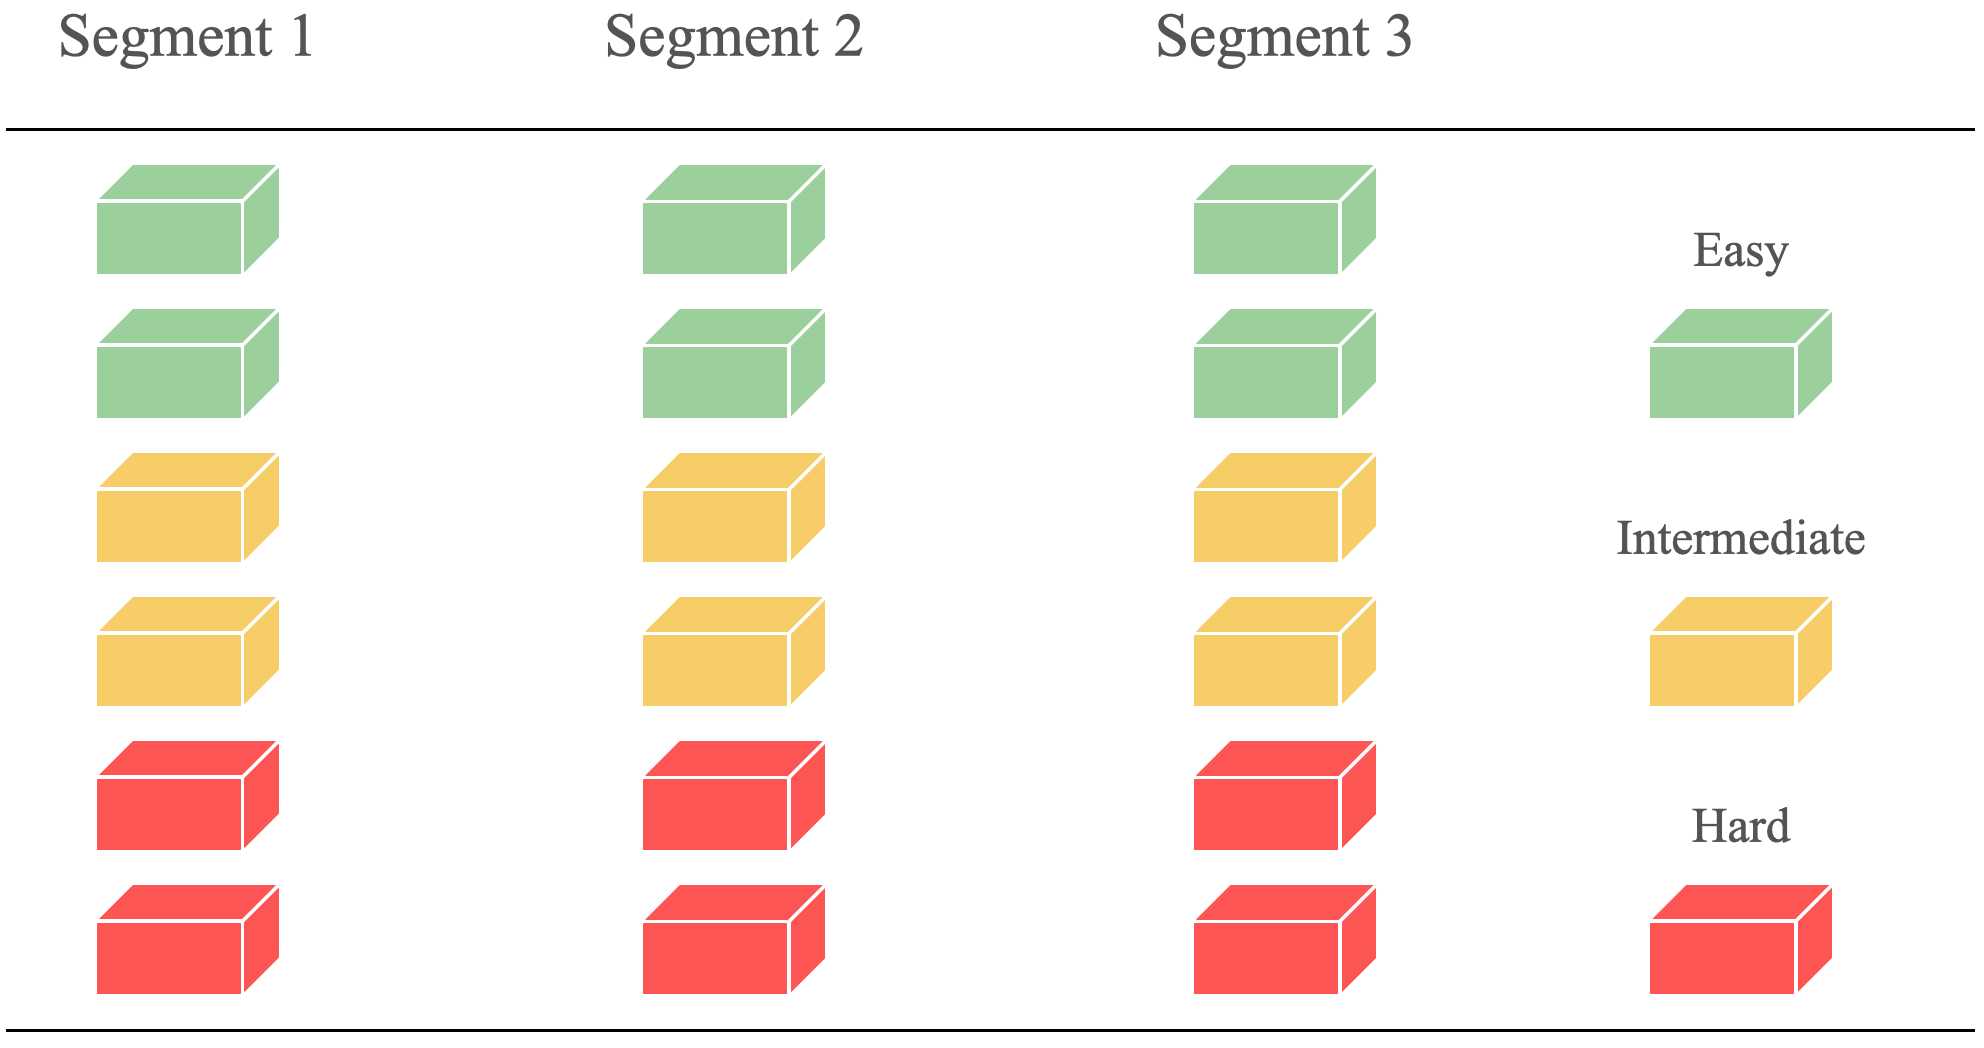
\includegraphics[scale=0.4]{experimental_setup}
\label{fig:experimental}
\end{figure}

The first segment emulated a scenario in which hostile spaceships approached the respondent's spaceship. The respondent was required to quickly react by defusing the hostiles in order to survive. The increment in difficulty caused the process of defusing hostile spaceships to become more challenging, hereby aiming to cause an increase in workload. The second segment emulated a scenario in which the respondent had to navigate their spaceship trough space, gathering as many way-points as possible. Obstacles around which the respondent had to navigate carefully, as well as hostile spaceships the respondent had to decimate, were introduced in the higher difficulty sessions. The third and final segment emulated a machine room, in which respondents had to control the power based on randomly generated requests. In the increased difficulty settings, variables that could overheat the spaceship were introduced, demanding the respondent to multi-task and aiming to increase workload as a consequence.

\subsubsection{Respondents}
In total, 25 respondents have participated in the study. No additional descriptive statistics can be presented in the this section as of yet. The respondents are students recruited from the University of Twente. Recruitment has been conducted by means of Sona, which is a cloud-based participant management system. A requirement for participation was that respondents didn't have any constraints that might interfere with the utilized sensors, such as for example a pacemaker. This was assessed by means of a short demographic questionnaire prior to the experiment. Additionally, respondents were made aware of informed consent prior to the experiment in order to ensure completely voluntary participation. Respondents were able to draw back from the experiment at any time. 

\subsubsection{Devices and Sampling Rate}
The Shimmer3 GSR+ sensor was used for both PPG and GSR measurements. This device was worn on the wrist. Signals were communicated wirelessly. An ear-clip was utilized for measuring PPG, and converting this to estimate heart rate. Skin conductivity, or GSR, was monitored by two electrodes attached to the fingers \cite{shimmer}. EEG measurement was conducted with the Muse 2, which is a multi-sensor headband that provides feedback on brain activity \cite{muse}. The Shimmer3 GSR+ is able to read and output data signals on a sampling rate of 256 Hz, whereas the Muse 2 is able to sample at a maximum rate of 220 Hz. 

As was set forth in the introduction, real-time classification requires a swiftly classifying network. A higher sampling rate equals more data traveling through the network, decelerating classification speed. As a consequence, it is highly beneficial to input data on the minimum required sampling rate with which key features can be detected consistently.

\citeA{fujita2019evaluation} explored the required sampling rate for PPG feature detection. The extent to which important features were detected was contrasted for several sampling rates. A sampling rate of 60 Hz was found to be the absolute minimum required sampling rate for extracting all commonly utilized features in a stable manner \cite{fujita2019evaluation}. Utilizing a slightly higher sampling rate is the safer option, however. The Shimmer3 GSR+ manufacturers recommend a sampling rate of 100 Hz for PPG \cite{shimmer}. Hence, a sampling rate of 100 Hz was specified for the PPG modality. 

The required sampling rate for the GSR modality is substantially lower as compared with both PPG and EEG measurement. In fact, the Shimmer3 GSR+ manufacturers recommend a sampling rate ranging between 0.03 and 5 Hz \cite{shimmer}. A sampling rate of 5 Hz was specified as a consequence. 

For the EEG modality, different features require a widely different sampling rate in order to be detected. Frequency bands for traditionally considered EEG features reside on about 0.5-4 Hz for the delta feature, and at most on about 16-24 Hz for the beta feature. The gamma feature recently gained in popularity, and resides on a frequency band ranging up to 80 Hz \cite{weiergraeber2016sampling}. In order to be able to detect an EEG feature residing on a 80 Hz frequency band, a substantially higher sampling rate is required to record the signal without aliasing. The required sampling rate can be determined by means of the Nyquist criterion for practical EEG sampling, defined as Equation \ref{eqn:nyquist},

\begin{equation}
\label{eqn:nyquist}
f_{samp} > 2.5 * f_{max}
\end{equation}
where $f_{samp}$ reflects the required sampling rate and $f_{max}$ reflects the frequency band around which the feature to be detected resides \cite{srinivasan1998estimating}. Hence, in order to be able to detect the gamma feature stably, a sampling rate of $2.5*80=200$ was specified for the EEG modality. A summary of the specified sampling rates per modality are depicted in Table \ref{table:samplingrate}.

\bgroup
\def\arraystretch{1.6}%  
\begin{table}[h]
\bigskip
\caption{Sampling Rate per Modality}
\label{table:samplingrate}
\begin{tabular}{ll}
    & Specified sampling rate (Hz) \\ \hline
 Electroencephalogram (EEG) & 200                         \\
Galvanic Skin Response (GSR) & 5                           \\
Photoplethysmography (PPG) & 100                         \\ \hline
\end{tabular}
\end{table}
\bigskip
\egroup

\subsubsection{Synchronization}
Data streams stemming from the different modalities were required to be properly synchronized. This was accomplished by means of an application called Lab-Streaming Layer, hereafter referred to as "LSL". The data streams stemming from the different modalities were all streamed to LSL during the experiment. LSL properly synchronized these data streams, such that they are parallel. Subsequently, all data was recorded into a single file per participant \cite{kothe2018lab}.
\bigskip

\subsection{Framework Architecture}
The upcoming section opens with the description of the architecture of the three single-modular networks. Subsequently, the multi-modular network architecture is elaborated upon. Lastly, several variations made on this multi-modular architecture are discussed. 

\subsubsection{Single-modular Network: Architectures}
The appropriate architecture for each of the single-modular networks is determined by combining insights from the literature. The three single-modular network architectures are depicted as Figure \ref{fig:singlearchitecture}.

\begin{figure}
\caption{The Three Single-modular Network Architectures}
\bigskip
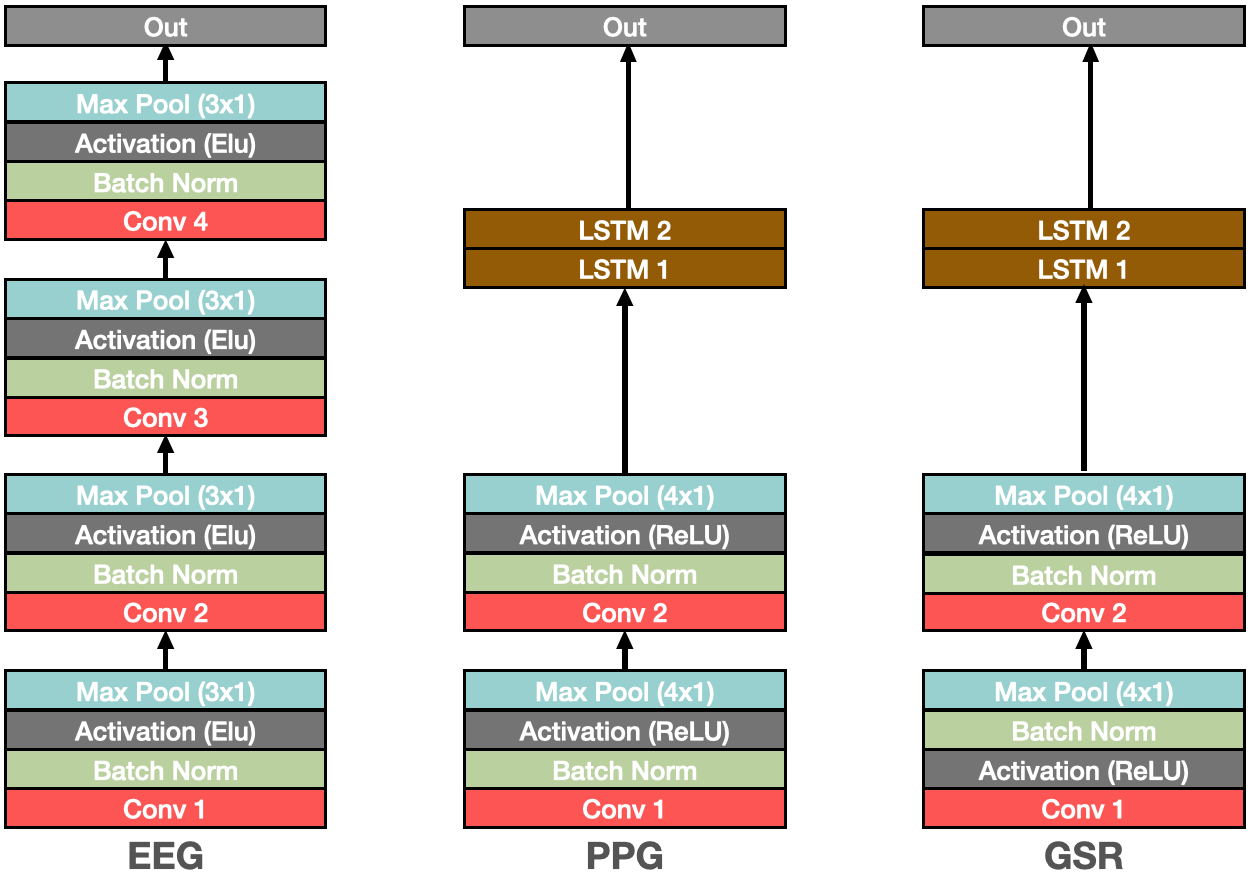
\includegraphics[scale=0.725]{single_model_architecture}
\label{fig:singlearchitecture}
\end{figure}

The utilized network for the EEG modality was a ConvNet as proposed by \citeA{schirrmeister2017deep}. The network was designed to include four convolutional blocks, each constituting a convolutional layer, followed by a batch normalization layer. The Exponential Linear Unit, hereafter referred to as "ELU", function was utilized as activation function. Each convolutional block was closed with a max pooling layer of stride three.

The utilized network for the GSR modality was a LSTM ConvNet hybrid, inspired from the work of \citeA{sun2019hybrid} and \citeA{dolmans2020perceived}. The network was designed to include two convolutional blocks, each constituting a convolutional layer, followed by a batch normalization layer, the activation layer and closed with a max-pooling layer of stride four. The Rectified Linear Unit, hereafter referred to as "ReLU", function was utilized as activation function. Following these two convolutional blocks were two LTSM layers.

Lastly, the utilized network for the PPG modality was inspired from the network as proposed by \citeA{biswas2019cornet}. The network opens with two convolutional blocks, each consisting of a convolutional layer, a batch normalization layer, the activation layer and closed with a max pooling layer of stride four. The utilized activation function was the ReLU. Following these convolutional blocks were two LTSM layers.

\subsubsection{Multi-modular Network: Architecture}
The network architecture utilized for the multi-modular approach was determined by a combination of the single-modular networks, as derived from the literature. The previously delineated design principles (i.e. the principles of modularity and generalizability) were taken into account when doing so. A visual representation of the multi-modular network is depicted as Figure \ref{fig:multiarchitecture}.

\begin{figure}
\caption{The Multi-modular Network Architecture}
\bigskip
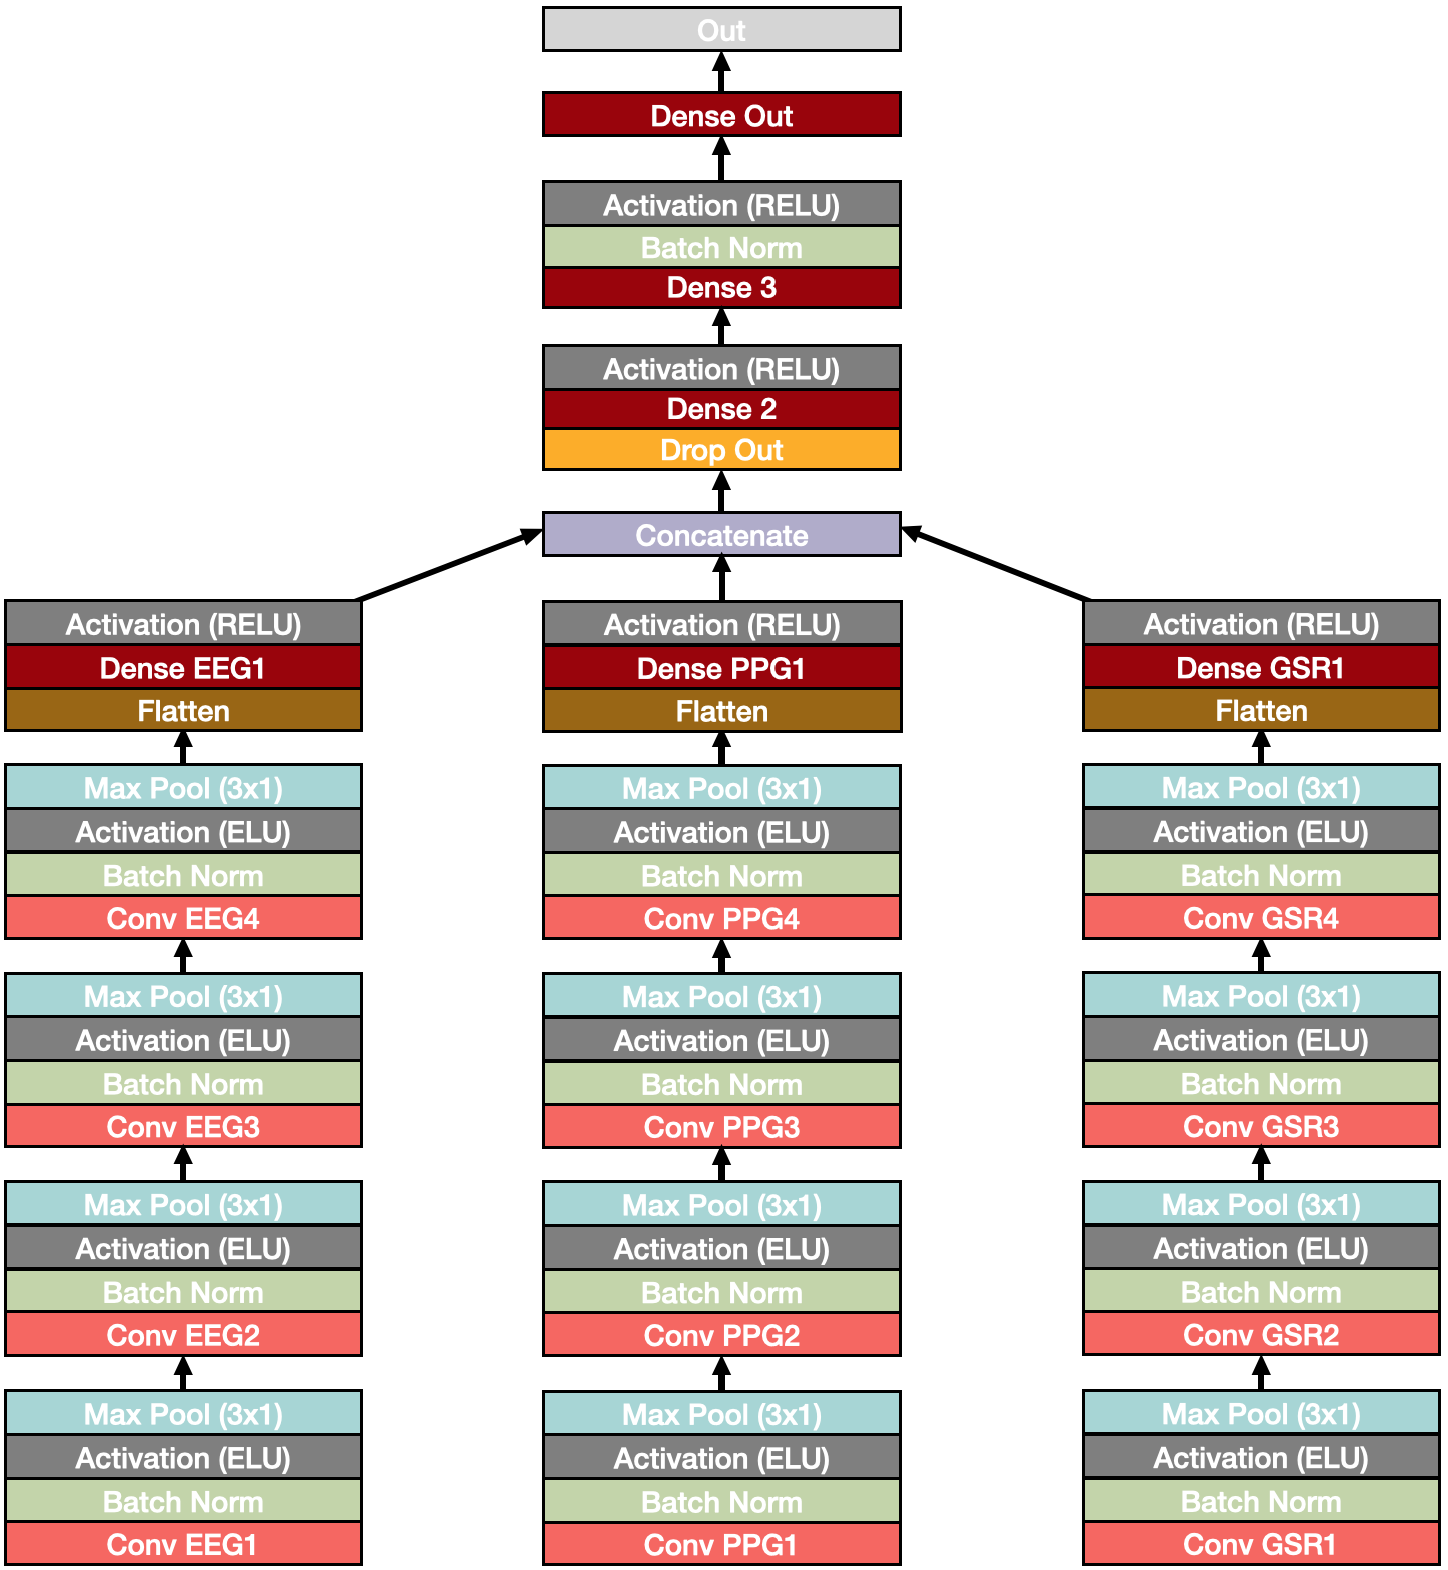
\includegraphics[scale=0.725]{multi_model_architecture}
\label{fig:multiarchitecture}
\end{figure}

An intermediate fusion strategy is adopted due to its highly flexible nature as compared with other fusion strategies. The architecture for the single-modular parts of the network remained unchanged. In order to fuse the  single-modular parts of the network, each of these is closed with one fully connected dense layer before feeding into the head network. This is done in order to flatten all inputs towards a lower dimensional space, such that concatenation was possible. The head network consists of four dense layers. These layers are alternated with a batch normalization and max-pooling layer with the objective of stabilization. 

\subsubsection{Multi-modular Network: Variations}
Speed is a potential bottleneck for a multi-modular approach that is destined to classify in real-time. The previously delineated network is substantially complex in nature, hence posing the risk of not being able to classify fast enough. Therefore, several variations on this network architecture have been designed. These variations are not made by altering the network architecture, for deviating from the validated architecture could be detrimental with regards to performance. Hence, three variations with regards to size of the network as depicted in Figure \ref{fig:multiarchitecture} have been considered. The goal was to propose a network that is fast enough for real-time classification, whilst maintaining the highest amount of accuracy as possible. 

Network size can be understood as the amount of specified filters for convolutional layers, and the amount of specified neurons for all other utilized layers. A decrease in the specified amount of filters and neurons constitutes a decrease in network size, and consequently a decrease in the amount of required calculations. Doing so was expected to bring about an increase in speed. An overview of all three multi-modular network variations, and the amount of specified neurons/filters per layer, is provided in Table \ref{table:modelvariations}. Network 1 is referred to as the full network. The size of this network was determined by consulting the literature. The sizes of each of the sub-parts, i.e. the EEG, PPG and GSR sub-parts, were roughly adopted from the research that proposed these designs initially. The size of Network 2 constitutes of 75 \% of the size of the full network. Lastly, Network 3 constitutes of 50 \% of the size of the full network.

\bgroup
\def\arraystretch{1.6}%  
\begin{table}[h]
\caption{Model Variations Based on Size}
\label{table:modelvariations}
\begin{tabular}{lllll}
\hline
        & EEG        & GSR        & PPG        & Head       \\ \hline
Network 1 & Conv1: 25  & Conv1: 128 & Conv1: 128 & Dense: 712 \\
        & Conv2: 50  & Conv2: 128 & Conv2: 128 & Dense: 356 \\
        & Conv3: 100 & LSTM1: 256 & LSTM1: 256 & Dense: 178 \\
        & Conv4: 200 & LSTM1: 256 & LSTM2: 256 &            \\ 
        \vspace{3ex}
        & Dense: 200 & Dense: 256 & Dense: 256 &            \\ \hline
Network 2 & Conv1: 18  & Conv1: 96  & Conv1: 96  & Dense: 534 \\
        & Conv2: 34  & Conv2: 96  & Conv2: 96  & Dense: 267 \\
        & Conv3: 75  & LSTM1: 192 & LSTM1: 192 & Dense: 134 \\
        & Conv4: 150 & LSTM1: 192 & LSTM1: 192 &            \\
        \vspace{3ex}
        & Dense: 150 & Dense: 192 & Dense: 192 &            \\ \hline
Network 3 & Conv1: 13  & Conv1: 64  & Conv1: 64  & Dense: 356 \\
        & Conv2: 25  & Conv2: 64  & Conv2: 64  & Dense: 178 \\
        & Conv3: 50  & LSTM1: 128 & LSTM1: 128 & Dense: 89  \\
        & Conv4: 100 & LSTM1: 128 & LSTM2: 128 &            \\
        & Dense: 100 & Dense: 128 & Dense: 128 &            \\ \hline
\end{tabular}
\vspace{2ex}

\begin{doublespacing}
{\raggedright \textit{Note:} For all convolutional layers the depicted number reflects the amount of utilized filters, whereas for LTSM layers it reflects the amount  of nodes. \par}
\end{doublespacing}
\end{table}
\egroup

\clearpage
\subsection{Model Evaluation}
The performance of the networks has been assessed and contrasted by means of several performance metrics. When assessing performance in deep/machine-learning, it is of importance to realize that each performance metric may favor one approach over the other, simply and solely due to the mathematical nature in which both the metric and the model are defined \cite{gunawardana2009survey}. For this reason, we deemed it of importance to not merely evaluate performance based on one or two metrics. The adopted approach is rather to consider a conglomerate of different metrics, and evaluate performance based on the whole span of those. The utilized metrics constitute six well known and widely deployed metrics in the field of deep/machine-learning. All six metrics are constructed from the confusion matrix. The theoretical format of the confusion matrix is depicted as Figure \ref{fig:confusion}.

\bigskip
\bgroup
\def\arraystretch{1.6}%  
\begin{figure}[h]
\caption{Confusion Matrix}
\label{fig:confusion}
\begin{tabular}{lll}
                                        & True Positive          & True Negative          \\ \cline{2-3} 
\multicolumn{1}{l|}{Predicted Positive} & \multicolumn{1}{l|}{a} & \multicolumn{1}{l|}{b} \\ \cline{2-3} 
\multicolumn{1}{l|}{Predicted Negative} & \multicolumn{1}{l|}{c} & \multicolumn{1}{l|}{d} \\ \cline{2-3} 
\end{tabular}
\end{figure}
\egroup
\bigskip

The six metrics include accuracy, sensitivity, specificity, positive predicted value hereafter referred to as "PPV, negative predicted value hereafter referred to as "NPV" and F1. Table \ref{table:metrics} depicts the mathematical composition of these performance metrics, by partly referring to confusion matrix depicted as Figure \ref{fig:confusion}. In substantive terms, accuracy can simply be understood as the proportion of correct classifications. Sensitivity is understood as the proportion true positives, whereas specificity is understood as the proportion of true negatives. PPV reflects the proportion of predicted positives that are correctly predicted as positive. NPV on the other hand reflects the proportion of predicted negatives that are correctly predicted to be negative. Lastly, F1-score is a function of both sensitivity and PPV, seeking balance between the latter two. 

\bgroup
\def\arraystretch{1.8}%  
\begin{table}[h]
\caption{Utilized Performance Metrics}
\label{table:metrics}
\begin{tabular}{ll}
\hline
Accuracy:                       & \(\frac{\!\!\!\!\!\!\!\!\!\!\!\!\!\!a+d}{a+b+c+d}\) \\
Sensitivity:                    & \(\frac{a}{a+c}\)                                   \\
Specificity:                    & \(\frac{d}{b+d}\)                                   \\
Positive Predicted Value (PPV): & \(\frac{a}{a+b}\)                                   \\
Negative Predicted Value (NPV):       & \(\frac{d}{c+d}\)                                   \\
F1-score:                     & \(\frac{2*Sensitivity*PPV}{Sensitivity+PPV}\)       \\ \hline
\end{tabular}
\end{table}
\egroup

For each of the three single-modular networks, as well as each of the three multi-modular network variants, these six metrics have been constructed and reported. The network that performed best across the range of these metrics was considered to be the superior performing network. In case of contradictory interpretations, a reference was made back to the mathematical definition and substantive interpretation of the previously delineated performance metrics. To summarize, with the described assessment approach it was aimed to gain insight into multiple dimension of network performance, resulting in a broad and complete assessment of performance altogether.     

\newpage
\bibliographystyle{apacite}
\bibliography{References}

\end{document}
